% Author: Izaak Neutelings (December 2021)
\documentclass[border=3pt,tikz]{standalone}
\usepackage{pgfplots}
\usepackage[siunitx]{circuitikz}
\usepackage[outline]{contour} % glow around text
\usetikzlibrary{arrows}
\usetikzlibrary{decorations.markings}
\tikzset{>=latex} % for LaTeX arrow head
\usepackage{xcolor}
\contourlength{1.5pt}

\colorlet{Icol}{blue!60!black}
\colorlet{Ccol}{orange!90!black}
\colorlet{Rcol}{green!50!black}
\colorlet{myred}{red!90!black}

\newcommand\EMF{\mathcal{E}}
\tikzstyle{EMF}=[battery1,l=$\EMF$,thin]
\tikzstyle{internal R}=[R,color=Rcol,Rcol,l=$r$,/tikz/circuitikz/bipoles/length=25pt]
\tikzstyle{thick R}=[R,color=Rcol,thick,Rcol,l=$R$,/tikz/circuitikz/bipoles/length=35pt]
\tikzstyle{small <->}=[{Latex[length=4,width=3]}-{Latex[length=4,width=3]},thick]
\def\tick#1#2{\draw[thick] (#1) ++ (#2:0.1) --++ (#2:-0.2)}


\begin{document}


% RESISTOR with EMF
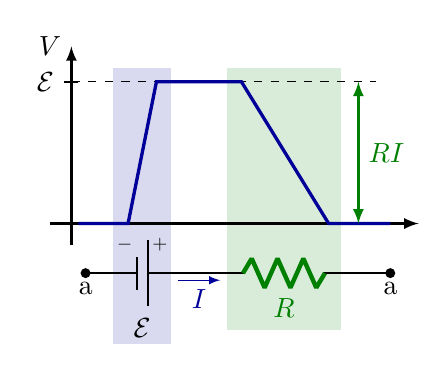
\begin{tikzpicture}[scale=0.9]
  
  \def\Vmax{2.0}
  
  % FILL AREA
  \fill[Icol!15] (0.09,-1.7) rectangle (0.90,\Vmax+0.2);
  \fill[Rcol!15] (1.70,-1.5) rectangle (3.30,\Vmax+0.2);
  
  % AXIS
  \begin{scope}[shift={(-0.5,0)}]
    \draw[->,thick]
      (-0.3,0) -- (4.9,0);
    \draw[->,thick]
      (0,-0.3) --++ (0,\Vmax+0.8) node[left] {$V$}; %\Delta
    \tick{0,\Vmax}{0} node[left] {$\EMF$};
    \draw[dashed]
      (0,\Vmax) --++ (4.3,0);
  \end{scope}
  
  % GRAPH
  \draw[very thick,Icol]
    (-0.4,0) -- (0.3,0)
    -- (0.7,\Vmax) -- (1.9,\Vmax)
    -- (3.13,0) -- (4.0,0);
  \draw[<->,thick,Rcol]
    (3.55,0) --++ (0,\Vmax) node[midway,right] {$RI$};
  
  % CIRCUIT
  \begin{scope}[shift={(0,-0.7)}]
    \draw[thick]
      (4,0) to[thick R] (1,0) 
            to[EMF] (0,0) -- (-0.3,0);
    \fill[black] (-0.3,0) circle (2pt) node[below] {a};
    \fill[black] (4,0) circle (2pt) node[below] {a};
    \node[scale=0.7] at (0.25,0.4) {$-$};
    \node[scale=0.7] at (0.75,0.4) {$+$};
    \draw[->,Icol] (1.0,-0.1) --++ (0.6,0) node[midway,below] {$I$};
  \end{scope}
  
\end{tikzpicture}


% RESISTOR with EMF + internal resistance
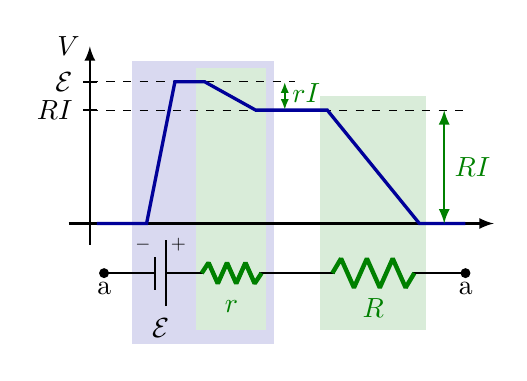
\begin{tikzpicture}[scale=0.9] %[x=30] %,y=100pt
  
  \def\Vmax{2.0}
  \def\RI{1.6}
  
  % FILL AREA
  \fill[Icol!15] (0.09,-1.7) rectangle (2.10,\Vmax+0.3);
  \fill[Rcol!15] (1.00,-1.5) rectangle (1.99,\Vmax+0.2);
  \fill[Rcol!15] (2.75,-1.5) rectangle (4.25,\RI+0.2);
  
  % AXIS
  \begin{scope}[shift={(-0.5,0)}]
    \draw[->,thick]
      (-0.3,0) -- (5.7,0);
    \draw[->,thick]
      (0,-0.3) --++ (0,\Vmax+0.8) node[left] {$V$}; %\Delta
    \tick{0,\Vmax}{0} node[left] {$\EMF$};
    \tick{0,\RI}{0} node[left] {$RI$};
    \draw[dashed]
      (0,\Vmax) --++ (2.9,0)
      (0,\RI) --++ (5.3,0);
  \end{scope}
  
  % GRAPH
  \draw[very thick,Icol]
    (-0.4,0) -- (0.3,0) -- (0.7,\Vmax)
    -- (1.12,\Vmax) -- (1.84,\RI)
    -- (2.85,\RI) -- (4.15,0) -- (4.8,0);
  \draw[small <->,Rcol]
    (2.25,\Vmax) --++ (0,\RI-\Vmax) node[pos=0.4,right=-1] {$rI$};
  \draw[<->,thick,Rcol]
    (4.5,0) --++ (0,\RI) node[midway,right] {$RI$};
  
  % CIRCUIT
  \begin{scope}[shift={(0,-0.7)}]
    \draw[thick]
      (4.8,0) to[thick R] (2.2,0) -- 
      (2.0,0) to[internal R] (1,0)
              to[EMF] (0,0) -- (-0.3,0);
    \fill[black] (-0.3,0) circle (2pt) node[below] {a};
    \fill[black] (4.8,0) circle (2pt) node[below] {a};
    \node[scale=0.7] at (0.25,0.4) {$-$};
    \node[scale=0.7] at (0.75,0.4) {$+$};
    %\draw[->,Icol] (I0)++(1.0, 0.1) --++ (1,0) node[midway,above] {$I_0$};
  \end{scope}
  
\end{tikzpicture}


% RESISTOR with EMF + series
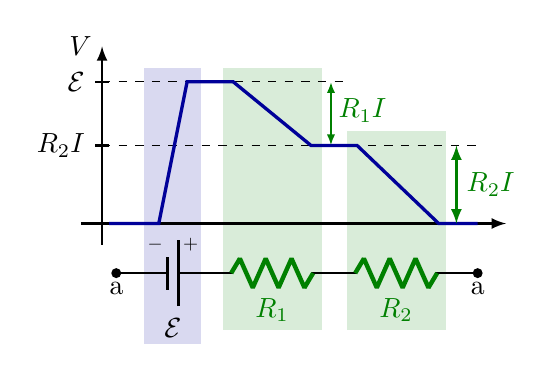
\begin{tikzpicture}[scale=0.9]
  
  \def\Vmax{2.0}
  \def\RI{1.1}
  
  % FILL AREA
  \fill[Icol!15] (0.09,-1.7) rectangle (0.90,\Vmax+0.2);
  \fill[Rcol!15] (1.20,-1.5) rectangle (2.60,\Vmax+0.2);
  \fill[Rcol!15] (2.95,-1.5) rectangle (4.35,\RI+0.2);
  
  % AXIS
  \begin{scope}[shift={(-0.5,0)}]
    \draw[->,thick]
      (-0.3,0) -- (5.7,0);
    \draw[->,thick]
      (0,-0.3) --++ (0,\Vmax+0.8) node[left] {$V$}; %\Delta
    \tick{0,\Vmax}{0} node[left] {$\EMF$};
    \tick{0,\RI}{0} node[left] {$R_2I$};
    \draw[dashed]
      (0,\Vmax) --++ (3.4,0)
      (0,\RI) --++ (5.3,0);
  \end{scope}
  
  % GRAPH
  \draw[very thick,Icol]
    (-0.4,0) -- (0.3,0) -- (0.7,\Vmax)
    -- (1.35,\Vmax) -- (2.45,\RI)
    -- (3.10,\RI) -- (4.25,0) -- (4.8,0);
  \draw[small <->,Rcol]
    (2.73,\Vmax) --++ (0,\RI-\Vmax) node[pos=0.45,right=-1] {$R_1I$};
  \draw[<->,thick,Rcol]
    (4.5,0) --++ (0,\RI) node[midway,right] {$R_2I$};
  
  % CIRCUIT
  \begin{scope}[shift={(0,-0.7)}]
    \draw[thick]
      (4.8,0) to[thick R,l=$R_2$] (2.5,0) -- 
      (2.5,0) to[thick R,l=$R_1$] (1.3,0) -- (1,0)
              to[EMF] (0,0) -- (-0.3,0);
    \fill[black] (-0.3,0) circle (2pt) node[below] {a};
    \fill[black] (4.8,0) circle (2pt) node[below] {a};
    \node[scale=0.7] at (0.25,0.4) {$-$};
    \node[scale=0.7] at (0.75,0.4) {$+$};
    %\draw[->,Icol] (I0)++(1.0, 0.1) --++ (1,0) node[midway,above] {$I_0$};
  \end{scope}
  
\end{tikzpicture}


% RESISTOR with EMF - parallel
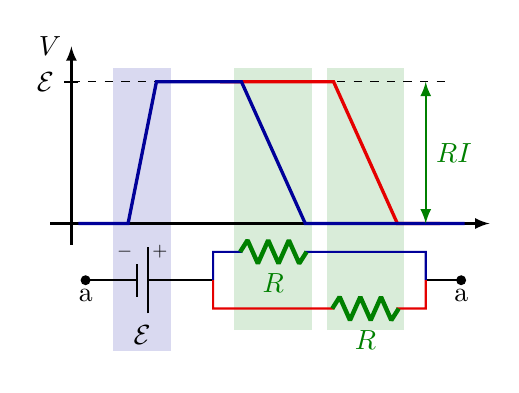
\begin{tikzpicture}[scale=0.9]
  
  \def\Vmax{2.0}
  
  % FILL AREA
  \fill[Icol!15] (0.09,-1.8) rectangle (0.90,\Vmax+0.2);
  \fill[Rcol!15] (1.80,-1.5) rectangle (2.90,\Vmax+0.2);
  \fill[Rcol!15] (3.10,-1.5) rectangle (4.20,\Vmax+0.2);
  
  % AXIS
  \begin{scope}[shift={(-0.5,0)}]
    \draw[->,thick]
      (-0.3,0) -- (5.9,0);
    \draw[->,thick]
      (0,-0.3) --++ (0,\Vmax+0.8) node[left] {$V$}; %\Delta
    \tick{0,\Vmax}{0} node[left] {$\EMF$};
    \draw[dashed]
      (0,\Vmax) --++ (5.3,0);
  \end{scope}
  
  % GRAPH
  \draw[very thick,myred]
    (1.6,\Vmax) -- (3.2,\Vmax)
    -- (4.1,0) -- (4.7,0);
  \draw[very thick,Icol]
    (-0.4,0) -- (0.3,0)
    -- (0.7,\Vmax) -- (1.9,\Vmax)
    -- (2.8,0) -- (5.05,0);
  \draw[<->,thick,Rcol]
    (4.5,0) --++ (0,\Vmax) node[midway,right] {$RI$};
  
  % CIRCUIT
  \begin{scope}[shift={(0,-0.8)}]
    \draw[thick]
      (5,0) -- (4.5,0)
      (1.5,0) -- (1,0) to[EMF] (0,0) -- (-0.3,0);
    \draw[Icol,thick]
      (4.5,0) |- (3.2,0.4) to[thick R,/tikz/circuitikz/bipoles/length=28pt]
      (1.5,0.4) -| (1.5,0);
    \draw[myred,thick]
      (4.5,0) -- (4.5,-0.4) to[thick R,/tikz/circuitikz/bipoles/length=28pt]
      (2.8,-0.4) -| (1.5,0);
    \fill[black] (-0.3,0) circle (2pt) node[below] {a};
    \fill[black] (5,0) circle (2pt) node[below] {a};
    \node[scale=0.7] at (0.25,0.4) {$-$};
    \node[scale=0.7] at (0.75,0.4) {$+$};
  \end{scope}
  
\end{tikzpicture}


\end{document}